\documentclass[11pt]{article}
\usepackage[a4paper,margin=0.90in]{geometry}
\usepackage{amsmath,amssymb,amsthm,mathtools}
\usepackage{booktabs,array}
\usepackage{graphicx}
\usepackage{xcolor}
\usepackage[hidelinks]{hyperref}
\usepackage{xurl}
\setlength{\emergencystretch}{2em}
\hypersetup{
  pdftitle={Lossless Calibration Is Stored Memory},
  pdfauthor={Lluis Eriksson},
  pdfsubject={Topological McMillan-degree and Wigner--Smith bounds for passive quantum networks}
}
\usepackage[nameinlink,capitalise]{cleveref}
\usepackage{microtype}

\newtheorem{theorem}{Theorem}[section]
\newtheorem{proposition}[theorem]{Proposition}
\newtheorem{lemma}[theorem]{Lemma}
\newtheorem{corollary}[theorem]{Corollary}
\theoremstyle{definition}
\newtheorem{definition}[theorem]{Definition}
\newtheorem{example}[theorem]{Example}
\theoremstyle{remark}
\newtheorem{remark}[theorem]{Remark}
\newtheorem{limitation}[theorem]{Limitation}

\newcommand{\C}{\mathbb{C}}
\newcommand{\T}{\mathbb{T}}
\newcommand{\D}{\mathbb{D}}
\newcommand{\diag}{\operatorname{diag}}
\newcommand{\rank}{\operatorname{rank}}
\newcommand{\ord}{\operatorname{ord}}
\newcommand{\tr}{\operatorname{tr}}
\newcommand{\op}{\mathrm{op}}
\newcommand{\dd}{\mathrm{d}}
\newcommand{\e}{\mathrm{e}}
\newcommand{\mcdeg}{\deg_{\mathrm{McM}}}

\title{Lossless Calibration Is Stored Memory:\\
A Topological McMillan-Degree and Wigner--Smith Law\\
for Passive Quantum Networks}
\author{Lluis Eriksson}
\date{13 September 2026\\Private corrected candidate; parent 10 August 2026}

\begin{document}
\maketitle

\begin{abstract}
How many internal state coordinates in a specified rational realization
are required to transmit prescribed quantum
noise channels without loss while suppressing all signal directions
elsewhere? We synthesize classical degree and phase-volume mechanisms into
an architecture-independent protected signal/loss formulation for finite
rational inner networks.  Let a causal rational inner scattering matrix
$\mathsf S$ have McMillan degree $n$, signal block $G$, and complementary loss
block $C$.  At distinct regular boundary frequencies $\zeta_j$, suppose that
$G(\zeta_j)$ is isometric on a $k_j$-dimensional input subspace.  If $G$ is a
strict contraction at one other boundary frequency, then
\[
  \sum_j k_j\leq n.
\]
Indeed, every lossless direction lies in $\ker C(\zeta_j)$; a nonzero maximal
minor of $C$ therefore has a zero of multiplicity at least $k_j$.  Exterior
powers of a minimal Blaschke--Potapov factorization show that no minor can
have more than $n$ zeros.  The same factorization yields the exact topological
delay identity
\[
 \frac1{2\pi}\int_{-\pi}^{\pi}\tr Q(\theta)\,\dd\theta
 =\mcdeg\mathsf S=n,
 \qquad Q=-\mathrm{i}\mathsf S^*\partial_\theta\mathsf S\succeq0.
\]
Here $\theta$ is the unit-circle/sample-delay coordinate; a physical
continuous-frequency interpretation requires a specified frequency map.
Thus lossless calibration multiplicity is bounded by integrated
Wigner--Smith delay and forces peak trace delay at least $\sum_jk_j$.  The
bound is attained by a $2m$-port family with $M$ prescribed roots of unity.
A Rouch\'e version preserves complex zero counts in disjoint pole-free
closed regions for rational inner perturbed transfers holomorphic on those
regions and satisfying a strict contour margin for the same loss minor,
while an explicit counterexample shows why pointwise approximate calibration
alone cannot imply a degree bound.  Applied to a previously constructed
irreducible six-port reservoir filter, the law counts $3S$ calibration zeros
and proves that its degree $3S+6$ lies within six states of the optimum among
finite rational inner completions with the same exact calibration data and a
strict stop, not merely among reducing comparators.  Its determinant gives an
exact trace-delay spectrum whose integral equals $3S+6$ and whose peak is
exponential. Under the specified stationary weak-coupling Markov model,
the rate interpretation counts $\sum_j k_j$ nodewise preserved input
dimensions at distinct frequencies. Numerical degree entries are analytic
formula values, not computed minimal realizations; quadrature and root audits
test the explicit family. Sources, current corrections and dated executions
are distinguished in the accompanying package.
\end{abstract}

\noindent\textbf{Keywords:} rational inner networks; McMillan degree;
Wigner--Smith time delay; passive quantum reservoirs; Blaschke--Potapov
factorization; transmission zeros.

\section{The question and the answer}

Passive filtering is attractive in quantum reservoir engineering because it
can reshape a bath without continuous active control.  It is nevertheless
not resource-free: a sharply selective passive response is stored in internal
modes and long dwell times.  Previous work established this trade only for a
particular scalar all-pass mechanism inside an irreducible multichannel
construction \cite{ErikssonReservoir2026}.  That left the main architectural
loophole open: could a completely different passive MIMO realization obey the
same lossless calibrations with much less memory?

The answer is no for causal finite-dimensional rational inner networks.  The
obstruction is topological rather than metric.  Exact transmission makes a
complementary loss minor vanish.  A rational inner transfer of McMillan degree
$n$ can supply at most $n$ zeros to any one minor.  The winding of its
determinant is the same integer $n$, and the corresponding phase derivative
is the trace of the Wigner--Smith lifetime matrix.  Consequently
\begin{equation}\label{eq:headline}
 \boxed{
  \text{lossless calibration charge}
  \ \leq\ \text{McMillan degree}
  \ =\ \text{integrated Wigner--Smith memory}.}
\end{equation}

The ingredients surrounding \eqref{eq:headline} are classical.  McMillan
degree originated in finite passive-network realization theory
\cite{McMillan1952}; rational lossless matrices admit finite
Blaschke--Potapov products \cite{Potapov1955,AlpayJorgensenLewkowicz2016}; and
the lifetime matrix goes back to Wigner and Smith
\cite{Wigner1955,Smith1960}.  Tangential interpolation and degree-constrained
MIMO interpolation are also mature subjects
\cite{BallKang1990,GallivanEtAl2004,BallBolotnikov2017}.  Our contribution is an explicit synthesis connecting
\emph{lossless directional calibration of a protected signal block} to a
\emph{topological degree and lifetime budget of every passive completion},
including multiplicity, sharpness and a robust analytic certificate.  We do
not claim a new factorization theorem or a new definition of time delay.

The result advances a resource-boundary programme developed across three
earlier manuscripts.  The first framed a Heisenberg cut through coherence
maintenance costs \cite{ErikssonCut2026}; the second showed a finite-degree
irreducible/reducible MIMO separation \cite{ErikssonMIMO2026}; the third
embedded that separation in a passive quantum reservoir and exposed a scalar
dwell-time price \cite{ErikssonReservoir2026}.  Here the comparator class
disappears: the lower bound applies to every rational inner architecture.

\paragraph{Contributions.}
\begin{enumerate}
 \item A calibration-charge theorem counts independent lossless directions,
 including several directions at the same frequency.
 \item A self-contained exterior-power proof bounds every minor by the full
 network's McMillan degree.
 \item An exact Wigner--Smith sum rule turns the algebraic count into an
 integrated and peak passive-memory lower bound.
 \item A $2m$-port family saturates the charge, integrated-trace and
 peak-trace inequalities for arbitrary positive integers $m,M$. It does not
 saturate the largest-proper-delay bound.
 \item A Rouch\'e certificate preserves the count under passive analytic
 perturbations; a degree-one example proves that sampled approximate
 calibration alone is insufficient.
 \item The irreducible reservoir family is re-audited with all $3S$
 calibration zeros.  Its degree is $3S+6$, within an additive six states of
 the universal optimum, and its delay integral and peak are computed exactly.
\end{enumerate}

\section{Passive transfer model}

We use the unit-disc convention.  Let $\mathsf S:\D\to\C^{N\times N}$ be a
rational inner function: it is rational and analytic in $\D$, has no pole at
the boundary points under discussion, and satisfies
\begin{equation}\label{eq:inner}
 \mathsf S(\zeta)^*\mathsf S(\zeta)=I_N,
 \qquad \zeta\in\T.
\end{equation}
Pure delays $z^q$ are causal in this convention.  A minimal state-space
realization has dimension $n=\mcdeg\mathsf S$.  For square rational inner
functions this integer also equals the degree, or boundary winding, of the
scalar inner function $\det\mathsf S$.

\paragraph{A fixed continuous-frequency convention and its state count.}
For a half-plane interpretation choose $\kappa>0$ and a rotation $\phi$
so that $-e^{\mathrm{i}\phi}$ is none of the finitely prescribed calibration
or stop nodes, and set
\begin{equation}\label{eq:cayleymap}
 z_\kappa(s)=e^{\mathrm{i}\phi}\frac{\kappa-s}{\kappa+s},
 \qquad \Xi(s)=\mathsf S(z_\kappa(s)),\qquad \Re s>0.
\end{equation}
The map sends the right half-plane into $\D$; the rational transfer $\Xi$
is proper and stable, with unitary imaginary-axis values. An invertible
M\"obius substitution preserves McMillan degree, so $\mcdeg\Xi=n$.
Use Laplace transfer $\Xi(s)$ with an $e^{-\mathrm{i}\omega t}$ harmonic,
hence $s=-\mathrm{i}\omega$ and
$\theta=\phi+2\arctan(\omega/\kappa)$ modulo $2\pi$. The chain rule gives
\begin{equation}\label{eq:physicaldelay}
 Q_\omega=-\mathrm{i}\Xi(-\mathrm{i}\omega)^*
       \frac{\dd}{\dd\omega}\Xi(-\mathrm{i}\omega)
 =\frac{2\kappa}{\kappa^2+\omega^2}Q(\theta),\qquad
 \frac1{2\pi}\int_{\mathbb R}\tr Q_\omega\,\dd\omega=n.
\end{equation}
Here $Q_\omega$ has time units when $\omega$ and $\kappa$ have inverse-time
units; the dimensionless peak bound is not a fixed bound in seconds
independent of this chosen map.

The physical mode interpretation additionally requires an annihilation-only
passive realization
\[
 \Xi(s)=D_c+C_c(sI-A_c)^{-1}B_c,\quad
 A_c=-\mathrm{i}\Omega-\tfrac12C_c^*C_c,\quad
 B_c=-C_c^*D_c,\quad D_c^*D_c=I,\quad \Omega=\Omega^*.
\]
For a minimal realization of this form, $n$ is the number of complex
annihilation coordinates (oscillator modes), or $2n$ real quadratures;
extra unobservable modes do not count toward the minimal transfer degree.
These are the passive realization conditions and minimality convention of
\cite[\S\S3.1--3.3, Theorem~3.5]{GoughZhang2015}. The algebraic theorem does
not assert that a particular laboratory device has been synthesized or
that an arbitrary propagation-delay implementation has this finite mode
count. For the discrete-time interpretation, $n$ instead counts minimal
sample-delay state coordinates. All physical mode claims here are conditional
on the specified finite passive realization, with all loss ports included.

Select $m$ signal input columns, $p$ protected output rows and the remaining
$\ell=N-p$ loss-output rows.  With irrelevant blocks suppressed, write
\begin{equation}\label{eq:partition}
 \mathsf S(z)=
 \begin{pmatrix}
   G(z)& *\\ C(z)& *
 \end{pmatrix},
 \qquad
 G(z)\in\C^{p\times m},\quad C(z)\in\C^{\ell\times m}.
\end{equation}
Column unitarity gives, on every regular boundary point,
\begin{equation}\label{eq:defect}
 G(\zeta)^*G(\zeta)+C(\zeta)^*C(\zeta)=I_m.
\end{equation}
This equality is the only quantum-network identity used in the degree
obstruction.  It is also the standard preservation law behind passive linear
quantum input--output models
\cite{GoughJames2009,GoughZhang2015,NurdinEtAl2016}.

\begin{definition}[Calibration charge]\label{def:charge}
At a regular point $\zeta\in\T$, the lossless calibration space is
\[
 E_\zeta:=\ker\!\left(I_m-G(\zeta)^*G(\zeta)\right),
 \qquad k_\zeta:=\dim E_\zeta.
\]
For distinct calibration nodes $\zeta_1,\ldots,\zeta_M$, their total charge is
$K:=\sum_{j=1}^M k_{\zeta_j}$.
\end{definition}

The definition asks only for norm preservation.  It does not require a
specified output phase, a common invariant channel, reciprocity or
commutativity.  From \eqref{eq:defect},
\begin{equation}\label{eq:kernelidentity}
 E_\zeta=\ker C(\zeta).
\end{equation}
A \emph{strict stop} is one regular boundary point $\zeta_*\in\T$ for which
$\|G(\zeta_*)\|_{\op}<1$.  At such a point \eqref{eq:defect} makes
$C(\zeta_*)^*C(\zeta_*)$ positive definite.  In particular $\ell\geq m$ and
$C(\zeta_*)$ has full column rank.

\section{The minor-degree mechanism}

Two elementary lemmas carry the proof.  We include details because they make
the result easy to audit and expose exactly where rationality enters.

\begin{lemma}[Local nullity consumes determinant multiplicity]
\label{lem:nullity}
Let $A(z)$ be an $m\times m$ matrix holomorphic near $z_0$.  If
$\dim\ker A(z_0)\geq k$, then either $\det A\equiv0$ or
\begin{equation}\label{eq:nullityorder}
 \ord_{z_0}\det A\geq k.
\end{equation}
\end{lemma}

\begin{proof}
Choose a constant invertible input change of basis whose first $k$ columns
span a subspace of $\ker A(z_0)$.  The first $k$ columns of the transformed
matrix vanish at $z_0$, so every entry in those columns is divisible by
$z-z_0$.  Multilinearity of the determinant supplies at least $k$ factors.
Constant basis changes alter the determinant only by a nonzero constant.
\end{proof}

\begin{lemma}[Every minor inherits the full McMillan budget]
\label{lem:minordegree}
Let $\mathsf S$ be an $N\times N$ rational inner function of McMillan degree
$n$.  Every nonzero $r\times r$ minor of $\mathsf S$ has at most $n$ finite
zeros, counted with multiplicity and restricted to points where the minor is
regular.
\end{lemma}

\begin{proof}
A minimal finite Blaschke--Potapov factorization has exactly $n$ rank-one
factors. Precisely, use \cite[Theorem~3.1, square case Eq.~(3.5)]{AlpayJorgensenLewkowicz2016}.
That reference permits either pole region and writes elementary scalar factors
$(1-\bar a z)/(z-a)$. Apply its Schur-stable exterior-disc form to
$S^\#(z)=S(1/\bar z)^*$ and paraconjugate back: product order reverses,
McMillan degree is preserved, and the scalar factors become
$b_a(z)=(z-a)/(1-\bar a z)$ with $|a|<1$ (including $a=0$).
This supplies a minimal product of exactly $n$ rank-one factors in our
analytic-disc convention, rather than an arbitrary mixed-pole product in
which cancellations may occur:

\begin{equation}\label{eq:potapov}
 \mathsf S(z)=U\prod_{q=1}^{n}
 \left[I_N+\bigl(b_{a_q}(z)-1\bigr)u_qu_q^*\right],
 \quad
 b_a(z)=\frac{z-a}{1-\bar a z},\quad |a|<1,
\end{equation}
where $U$ is constant unitary and $\|u_q\|=1$.  Factors with $a_q=0$
include integer delays.

Every $r\times r$ minor is an entry of the exterior-power matrix
$\bigwedge^r\mathsf S$.  On $\bigwedge^r\C^N$, a factor in
\eqref{eq:potapov} becomes
\[
 I+\bigl(b_{a_q}(z)-1\bigr)P_q,
\]
where $P_q$ is the orthogonal projection onto wedges containing $u_q$.
Thus every entry of the product has a common scalar denominator dividing
$\prod_{q=1}^n(1-\bar a_qz)$ and a numerator of degree at most $n$.
Cancellation can only lower the degree.  A nonzero entry therefore has at
most $n$ finite zeros.
\end{proof}

The exterior-power argument is one proof choice, not an essential new
degree principle. Classical realization theory supplies a direct alternative.
Write a disc realization with $n$ states as
$T(z)=D+zC_r(I-zA)^{-1}B$. For row and column sets $I,J$ of equal size,
\[
 \det T_{I,J}(z)=
 \frac{\det\begin{pmatrix}I-zA&-zB_J\\(C_r)_I&D_{I,J}\end{pmatrix}}
 {\det(I-zA)}.
\]
Only the top $n$ rows of the numerator depend on $z$, each linearly, so its
degree is at most $n$. Cancellation can only lower it. This is the same
minor budget. The block determinant step is the Schur-complement identity
for the classical Rosenbrock system matrix: see
\cite[Section~1, Eq.~(1) and its following transfer-function formula]{DopicoQuintanaVanDooren2022},
with $T=I-zA$, $U=zB_J$, $V=(C_r)_I$ and $W=D_{I,J}$ in that reference's
notation. The displayed row-degree argument supplies the minor corollary
directly; we do not attribute a separately named calibration theorem to that
reference. The classical zero/pole degree-sum framework is reviewed in
\cite[Theorem~1 and Section~3]{DopicoQuintanaVanDooren2022}. The passive
completion identity supplies the subsequent interpretation as calibration
charge; neither scalar zero counting nor system-matrix theory is new here.

\section{Universal calibration-charge theorem}

The zero-budget and phase-volume mechanisms are classical and shared with
the spectral-routing formulation \cite{ErikssonRouting2026}. The contribution
here is their protected signal/loss formulation, nodewise calibration data,
qualified rational-inner robustness, saturation examples and six-port
application; no new factorization or independent-priority claim is made.


\begin{theorem}[Lossless calibration is stored degree]
\label{thm:charge}
Let $\mathsf S$ be a causal $N\times N$ rational inner transfer of McMillan
degree $n$, partitioned as in \eqref{eq:partition}.  Let
$\zeta_1,\ldots,\zeta_M\in\T$ be distinct regular calibration nodes with
charges $k_j=\dim E_{\zeta_j}$.  If there exists a regular strict-stop point
$\zeta_*\in\T$ satisfying $\|G(\zeta_*)\|_{\op}<1$, then
\begin{equation}\label{eq:chargebound}
 K:=\sum_{j=1}^M k_j\leq \mcdeg\mathsf S=n.
\end{equation}
\end{theorem}

\begin{proof}
At the strict stop, $C(\zeta_*)$ has full column rank.  Select $m$ of its rows
whose square submatrix $C_I(\zeta_*)$ has nonzero determinant, and put
$f(z)=\det C_I(z)$.  Hence $f\not\equiv0$.

At node $\zeta_j$, \eqref{eq:kernelidentity} gives
$E_{\zeta_j}\subseteq\ker C_I(\zeta_j)$, so
$\dim\ker C_I(\zeta_j)\geq k_j$.  By Lemma~\ref{lem:nullity}, $f$ has a zero of
multiplicity at least $k_j$ there.  The nodes are distinct, whence $f$ has at
least $K$ zeros counting multiplicity.  It is an $m\times m$ minor of
$\mathsf S$, so Lemma~\ref{lem:minordegree} gives $K\leq n$.
\end{proof}

\begin{remark}[Why the strict stop is necessary]
If $G$ is isometric everywhere, then $C\equiv0$ and every loss minor vanishes
identically; a constant unitary signal route has degree zero and arbitrarily
many lossless ``calibrations.''  One strict stop certifies that the chosen
minor is not the zero function.  The theorem is therefore a selectivity law,
not a charge for transparent wiring.
\end{remark}

\begin{remark}[No hidden architecture comparator]
The proof permits arbitrary frequency-dependent channel mixing, arbitrary
constant unitary pre- and post-processing, nonreciprocal inner networks, and
any number $\ell\geq m$ of loss outputs.  It compares neither with a reducing
class nor with a fixed numerator denominator bidegree.  This is the precise
sense in which \cref{thm:charge} closes the main loophole left by the earlier
architecture separation \cite{ErikssonReservoir2026}.
\end{remark}

\section{Topological Wigner--Smith memory law}

For $\zeta=\e^{\mathrm{i}\theta}$ define the dimensionless Wigner--Smith
matrix
\begin{equation}\label{eq:Qdef}
 Q(\theta):=-\mathrm{i}\,\mathsf S(\e^{\mathrm{i}\theta})^*
 \frac{\dd}{\dd\theta}\mathsf S(\e^{\mathrm{i}\theta}).
\end{equation}
In a physical frequency variable $\omega$, multiplication by
$\dd\theta/\dd\omega$ restores units of time.  The sign in
\eqref{eq:Qdef} matches the analytic-disc convention; changing to a
$z^{-1}$ engineering convention reverses the orientation and requires the
corresponding sign change.

\begin{theorem}[Degree is Wigner--Smith phase volume]
\label{thm:sumrule}
For a causal rational inner $\mathsf S$ of McMillan degree $n$,
\begin{equation}\label{eq:sumrule}
 Q(\theta)\succeq0,
 \qquad
 \frac1{2\pi}\int_{-\pi}^{\pi}\tr Q(\theta)\,\dd\theta
 =\operatorname{wind}_{\T}\det\mathsf S=n.
\end{equation}
\end{theorem}

\begin{proof}
For a single factor
$E_q=I+(b_{a_q}-1)u_qu_q^*$ in \eqref{eq:potapov}, direct differentiation
gives a rank-one positive delay
\begin{equation}\label{eq:poisson}
 Q_{E_q}(\theta)=
 \frac{1-|a_q|^2}{|\e^{\mathrm{i}\theta}-a_q|^2}\,u_qu_q^*,
\end{equation}
whose trace integrates to $2\pi$.  If $A$ and $B$ are inner, the product rule
is
\[
 Q_{AB}=B^*Q_AB+Q_B.
\]
Positivity therefore survives the entire Potapov product, and trace
invariance under unitary conjugation makes the integrated traces add to
$2\pi n$.

Equivalently, cyclicity of trace gives
$\tr Q=-\mathrm{i}\,\partial_\theta\log\det\mathsf S$.  Each rank-one
factor has determinant $b_{a_q}$, so $\det\mathsf S$ winds $n$ times.
\end{proof}

Combining the two theorems yields the operational statement.

\begin{corollary}[Universal memory budget]
\label{cor:memory}
Under the hypotheses of \cref{thm:charge},
\begin{equation}\label{eq:memorybudget}
 K\leq n
 =\frac1{2\pi}\int_{-\pi}^{\pi}\tr Q(\theta)\,\dd\theta
 \leq \sup_\theta\tr Q(\theta).
\end{equation}
Moreover,
\begin{equation}\label{eq:properdelay}
 \sup_\theta\lambda_{\max}(Q(\theta))\geq\frac{K}{N}.
\end{equation}
Consequently a uniform proper-delay cap $Q(\theta)\preceq D I_N$ permits at
most $K\leq ND$ units of lossless calibration charge.
\end{corollary}

The lower bound concerns phase volume, not only a single resonant peak.  A
network may distribute the required memory broadly over frequency or
concentrate it into sharp long-lived modes, but it cannot remove the integral.
This distinction complements the earlier scalar stopband theorem, which
forced an exponentially high peak for one particular suppression mechanism
\cite{ErikssonReservoir2026}.

\section{Sharpness at every dimension}

The coefficient one in \eqref{eq:chargebound} cannot be improved.

\begin{proposition}[Exact saturation]
\label{prop:sharp}
For every pair of integers $m,M\geq1$ there is a causal $2m$-port rational inner transfer with
$M$ distinct nodes, charge $m$ at each node, a perfect stop, and
\begin{equation}\label{eq:sharp}
 \mcdeg\mathsf S=mM=\sum_{j=1}^{M}k_j.
\end{equation}
Its Wigner--Smith trace is the constant $mM$, so the integrated bound and the
peak-trace bound are also equalities.
\end{proposition}

\begin{proof}
Let
\[
 H_m=\frac1{\sqrt2}\begin{pmatrix}I_m&I_m\\I_m&-I_m\end{pmatrix},
 \qquad
 \mathsf S_{m,M}(z)=H_m\diag(I_m,z^M I_m)H_m.
\]
Then
\begin{equation}\label{eq:sharpblocks}
 G(z)=\frac{1+z^M}{2}I_m,
 \qquad C(z)=\frac{1-z^M}{2}I_m.
\end{equation}
At every $M$th root of unity, $C=0$ and $k_j=m$.  At every solution of
$z^M=-1$, $G=0$.  Since $\det\mathsf S=z^{mM}$, its McMillan degree is $mM$.
Constant conjugation of $\diag(0,MI_m)$ gives $Q$, so $\tr Q=mM$.
\end{proof}

This saturating family is reducible and deliberately simple.  It proves that
irreducibility is not needed for the universal resource law.  Irreducibility
becomes useful for attaining strong stopband performance under richer
directional calibrations, as revisited in \cref{sec:irreducible}. Here the
proper-delay eigenvalues are $0$ and $M$, each $m$ times, whereas $K/N=M/2$.
Thus \eqref{eq:properdelay} is not saturated. No equality for arbitrary
prescribed node geometry or arbitrary port partitions is claimed.

\section{What robustness is possible---and what is not}

Exact boundary equalities are experimentally idealized.  Two different
notions of robustness must be separated.

\subsection{Analytic zero-count stability}

Let $f_0$ be the nonzero loss minor selected in the proof of
\cref{thm:charge}. Choose positively oriented Jordan contours
$\Gamma_1,\ldots,\Gamma_M$ whose closed interiors are pairwise disjoint.
Require $f_0$ to be holomorphic on a neighborhood of every closed interior,
with no zero on the contour, and let the interior of $\Gamma_j$ contain
$\zeta_j$ with multiplicity at least $k_j$. In particular, reference poles
are excluded from the entire enclosed regions, not just their boundaries.

\begin{theorem}[Rouch\'e-stable calibration charge]
\label{thm:rouche}
Under the preceding pole-free, disjoint-region hypotheses, let
$\widetilde{\mathsf S}$ be another rational inner transfer holomorphic on
a neighborhood of every closed interior, and let $\widetilde f$ denote
the same loss minor. If
\begin{equation}\label{eq:rouche}
 \sup_{z\in\Gamma_j}|\widetilde f(z)-f_0(z)|
 <\inf_{z\in\Gamma_j}|f_0(z)|
 \qquad(j=1,\ldots,M),
\end{equation}
then
\begin{equation}\label{eq:robustdegree}
 \mcdeg\widetilde{\mathsf S}\geq\sum_{j=1}^{M}k_j.
\end{equation}
More generally the right side may be replaced by the total number of zeros
of $f_0$ inside the contours, counted with multiplicity.
\end{theorem}

\begin{proof}
Rouch\'e's theorem \cite{Ahlfors1979} gives the same zero count for $f_0$ and
$\widetilde f$ inside each contour.  Their interiors are disjoint, so
$\widetilde f$ has at least $\sum_jk_j$ zeros.  Apply
Lemma~\ref{lem:minordegree} to $\widetilde{\mathsf S}$.
\end{proof}

The reference holomorphy condition cannot be dropped. For
$f_0=3(z-1)/(2(z-2))$, obtained from the two-port completion with
$b_{1/2}(z)=(z-1/2)/(1-z/2)$, the calibration charge is one. The constant
swap completion has $\widetilde f=1$ and degree zero. On $|z|=10$,
$\sup|1-f_0|\leq11/16<9/8\leq\inf|f_0|$, but the reference pole $z=2$
is enclosed; meromorphic zero-minus-pole counting does not give the asserted
degree bound. The corrected assumptions exclude this example. Likewise,
disjoint curves alone can be nested; disjoint interiors prevent double counts.

Preserved complex zeros need not stay on the real-frequency boundary.
Consequently this theorem does not guarantee nearby exact lossless boundary
calibrations after perturbation.

This is a robust \emph{model certificate}: it uses a rational fit or analytic
component model on small complex-frequency contours.  It does not pretend
that off-axis transfer values are direct laboratory observables.  In
practice, one fits a passive rational model to real-frequency scattering
data, propagates parameter uncertainty to \eqref{eq:rouche}, and verifies the
zero count on the model family.

\subsection{Why pointwise approximate calibration is insufficient}

\begin{proposition}[No count from unseparated approximate samples]
\label{prop:approxnogo}
Fix any positive integer $M$ and tolerance $\delta>0$.
There is a degree-one two-port rational inner transfer, $M$ distinct boundary
nodes, and a perfect stop such that the signal magnitude at every node is at
least $1-\delta$.
\end{proposition}

\begin{proof}
For $0<r<1$ set
\[
 b_r(z)=\frac{z-r}{1-rz},\qquad
 \mathsf S_r(z)=H_1\diag(1,b_r(z))H_1,
 \qquad G_r(z)=\frac{1+b_r(z)}2.
\]
This network has degree one and $G_r(-1)=0$.  Continuity and $G_r(1)=1$ give
an open boundary arc around $1$ on which $|G_r|\geq1-\delta$.  Select any $M$
distinct nodes in that arc.
\end{proof}

Thus a theorem depending only on the number of approximate samples is false:
the nodes may oversample one degree-one pass window.  Valid finite-tolerance
bounds need additional information---for example node separation plus a
derivative budget, or the analytic contour margin in \cref{thm:rouche}.  This
no-go prevents a common but serious overinterpretation of exact root counts.

\section{Near-optimal irreducible quantum reservoir filter}
\label{sec:irreducible}

We now apply the universal law to the explicit six-port family of
\cite{ErikssonReservoir2026}. Every use of irreducibility here is conditional on the cited companion theorem;
we do not give a new self-contained irreducibility proof. The imported result is as follows:
the theorem entitled ``Passive irreducible/reducing separation'' in that
reference, item~4, proves it whenever the stated stop bound is below one.
More precisely, its Section~4 theorem
``Passive irreducible/reducing separation'', item~4, uses $3(S-1)$
selected nodes in the open pass arc $|\theta|<\pi/6$. Its node-count lemma
selects $S-1$ solutions of $B_g(z)=1$ per group from the same scalar arms
and phases used below. These are a subset of the $S$ roots per group counted
here, with the same signatures $v_{g,z}=U(z)e_g$ and delayed calibration.
The companion's stop envelope on $5\pi/6\leq|\theta|\leq\pi$ is
$\varepsilon_S=(\pi S/6+1/2)e^{-9S/20}<1$ for every $S\geq5$:
it is below one at $S=5$, and its logarithmic derivative is
$1/(S+3/\pi)-9/20<0$ thereafter. Thus its item~4 applies to this family.
That argument uses the selected full-spark subset and a rational bidegree
ceiling; the present $3S$ charge counts all roots and does not assume full
spark of the entire enlarged set. Neither irreducibility nor that architectural comparison is
needed for the universal calibration-charge bound proved here.  The purpose is not to repeat its architectural
separation, but to answer a question that paper could not: how far is its
internal dimension from the best \emph{arbitrary} passive architecture?

Fix $\alpha=9/20$ and an integer $S\geq5$, and put
\begin{equation}\label{eq:familyb}
 r_S=1-\e^{-\alpha S},\quad
 b_r(z)=\frac{z-r}{1-rz},\quad
 B_S(z)=\eta_S b_{r_S}(z)^S,
\end{equation}
where $\eta_S=1$ for odd $S$ and $-1$ for even $S$.  Hence $B_S(-1)=-1$.
Let $\phi_g=(g-1)(1-r_S)$ for $g=0,1,2$ and $B_g=\e^{\mathrm{i}\phi_g}B_S$.
With the $3\times3$ Fourier matrix $F$, define
\begin{equation}\label{eq:mixers}
 U(z)=F\diag(1,z,z^2)F^*,\qquad
 U_{\rm rev}(z)=F\diag(z^2,z,1)F^*.
\end{equation}
The balanced interferometers and the full network are
\begin{equation}\label{eq:network}
 W_g(z)=\frac12
 \begin{pmatrix}1+B_g(z)&1-B_g(z)\\1-B_g(z)&1+B_g(z)\end{pmatrix},
 \qquad
 \mathsf S_S=\diag(U,I_3)\,W\,\diag(U_{\rm rev},I_3),
\end{equation}
where $W$ places the three $W_g$ on signal/loss port pairs.  Every factor is
inner.  The signal and loss blocks from the three signal inputs are
\begin{align}
 G_S(z)&=U(z)\diag\!\left(\frac{1+B_0(z)}2,
 \frac{1+B_1(z)}2,\frac{1+B_2(z)}2\right)U_{\rm rev}(z),
 \label{eq:GS}\\
 C_S(z)&=\diag\!\left(\frac{1-B_0(z)}2,
 \frac{1-B_1(z)}2,\frac{1-B_2(z)}2\right)U_{\rm rev}(z).
 \label{eq:CS}
\end{align}

Each scalar degree-$S$ inner function $B_g$ takes the value one at exactly
$S$ simple points of $\T$.  The three root sets are disjoint because the
phases $\phi_g$ are distinct modulo $2\pi$.  At a root $z$ of $B_g-1$, the
input direction $v_{g,z}=U(z)e_g$ is lossless and obeys
$G_S(z)v_{g,z}=z^2v_{g,z}$.  Hence the total calibration charge is
\begin{equation}\label{eq:KS}
 K_S=3S.
\end{equation}
At $z=-1$ every $|1+B_g(-1)|/2<1$, so the signal block is strictly
contractive.  The universal theorem already forces degree at least $3S$.

The realized degree is exact, not an entrywise upper bound.  Since
$\det U=\det U_{\rm rev}=z^3$ and $\det W_g=B_g$,
\begin{equation}\label{eq:dets}
 \det\mathsf S_S(z)=z^6\prod_{g=0}^{2}B_g(z),
 \qquad
 \det C_S(z)=z^3\prod_{g=0}^{2}\frac{1-B_g(z)}2.
\end{equation}
Therefore
\begin{equation}\label{eq:nearoptimal}
 \mcdeg\mathsf S_S=3S+6=K_S+6.
\end{equation}
The six-state overhead is exactly the two frequency-dependent mixers.  Thus
the same device previously proved superior to every calibrated reducing
comparator is now certified within an additive six states of the best
possible finite rational inner network of \emph{any} architecture with the
same exact calibration nodes/directions and a strict stop.

The determinant also gives the complete trace delay:
\begin{equation}\label{eq:exacttrace}
 \tr Q_S(\theta)=6+3S
 \frac{1-r_S^2}{1-2r_S\cos\theta+r_S^2}.
\end{equation}
Consequently
\begin{equation}\label{eq:exactdelay}
 \frac1{2\pi}\int_{-\pi}^{\pi}\tr Q_S\,\dd\theta=3S+6,
 \qquad
 \max_\theta\tr Q_S(\theta)
 =6+3S\frac{1+r_S}{1-r_S}
 =6+3S(2\e^{\alpha S}-1).
\end{equation}
The area is the compulsory topological memory.  The exponentially high peak
is the additional price of concentrating the scalar all-pass phases sharply
enough to achieve exponential stop suppression.

\begin{figure}[htbp]
 \centering
 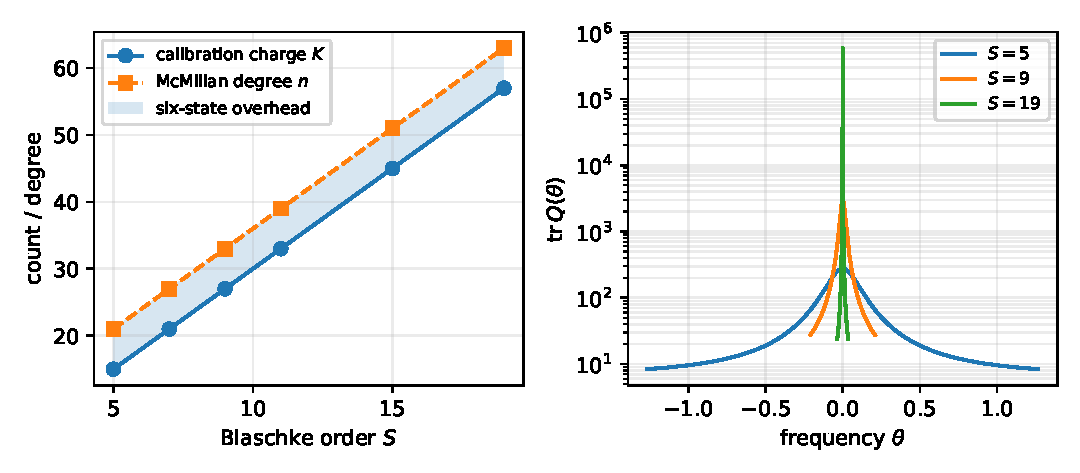
\includegraphics[width=0.94\linewidth]{figures/memory_law.pdf}
 \caption{Left: the explicit irreducible six-port construction has calibration
 charge $K_S=3S$ and analytically derived McMillan degree $n_S=3S+6$, a constant six-state
 overhead above the universal lower bound.  Right: the phase
 volume, fixed by the degree of each network and increasing from $21$ to
 $63$ across the shown family, becomes increasingly concentrated into a high Wigner--Smith peak as
 $r_S$ approaches the unit circle.  The frequency windows differ by $S$ so
 the peak shapes remain visible.}
 \label{fig:memory}
\end{figure}

\section{From scattering memory to decoherence selectivity}

The theorem is a network constraint. The following quantum-rate interpretation
is conditional on a stationary linear bath-transfer model and on the
weak-coupling assumptions needed to use its spectral matrix in a Markov
generator. Let the positive signal-input spectral matrix obey
\begin{equation}\label{eq:bath}
 j_-I_m\preceq J(\omega)\preceq j_+I_m,
 \qquad 0<j_-\leq j_+<\infty,
\end{equation}
and define the signal contribution to a Kossakowski matrix by
\begin{equation}\label{eq:koss}
 \Gamma_G(\omega)=G(\e^{\mathrm{i}\theta(\omega)})
 J(\omega)G(\e^{\mathrm{i}\theta(\omega)})^*.
\end{equation}
For completeness, let $b(t)$ be a stationary column of input bath
operators, let $J$ be the Fourier transform of its correlation matrix
$\langle b(t)b(0)^*\rangle$, and suppose the selected output is the linear
filter $y=h*b$ with Fourier transfer $G$. Inserting both convolutions
in $\langle y(t)y(0)^*\rangle$ and using stationarity gives the congruence
\eqref{eq:koss}. Independent auxiliary inputs contribute separate
positive spectral terms. The displayed matrix accounts only for the
signal input. Its use as a rate matrix at system Bohr frequencies requires
a specified system-bath coupling and the weak-coupling limit
\cite{Davies1974}; it is not derived from boundary unitarity alone.
Classical correlated-noise filter functions \cite{CerfontaineEtAl2021} are
related context, not a derivation of the quantum-port interface.

For any normalized lossless input $v\in\ker(I-G^*G)$, define the
output direction $w=Gv$. Then $\|w\|=1$ and $G^*w=v$, even when
$G$ is rectangular. Consequently
\begin{equation}\label{eq:passrate}
 w^*\Gamma_Gw=v^*Jv\geq j_-.
\end{equation}
This is a statement in the corresponding output direction, not an
identification of input and output spaces. In the square six-port example,
$Gv=z^2v$, so it also yields the same-direction statement.
At a stop where $\|G\|_{\op}\leq\varepsilon$,
\begin{equation}\label{eq:stoprate}
 \|\Gamma_G\|_{\op}\leq j_+\varepsilon^2.
\end{equation}
The spectral-rate contrast is therefore squared at the Kossakowski level.
The new statement is the compulsory resource behind preserving many pass
directions:
\begin{equation}\label{eq:quantummemory}
 K=\sum_{j=1}^{M}\dim E_{\zeta_j}
 \leq \mcdeg\mathsf S
 =\frac1{2\pi}\int\tr Q.
\end{equation}
The count is the sum of input-subspace dimensions at the distinct
calibration frequencies of Definition~2.1, not a single frequency-independent
dimension of global directions. Its interpretation as a statement about rates
remains conditional on the stationary weak-coupling Markov model specified
above; the underlying degree bound is a deterministic transfer-matrix result.

Auxiliary vacuum ports remain physical channels.  They can add a baseline to
an observed Ramsey decay, as accounted for explicitly in
\cite{ErikssonReservoir2026}; \cref{thm:charge} neither removes nor hides that
floor.  What it proves is orthogonal: regardless of how the passive network is
realized, exact preservation of $K$ selected spectral directions together
with any strict all-direction stop requires at least $K$ internal-state
degrees and the same amount of integrated delay.

This is also the precise connection to the Heisenberg-cut resource viewpoint
\cite{ErikssonCut2026}.  Active maintenance can pay in work and entropy
production; a passive architecture can avoid that continuous drive, but its
selective boundary conditions are stored as dynamical memory.  No universal
conversion from McMillan degree to joules is asserted: such a conversion
depends on linewidths, temperature, fabrication and initialization.  The
universal statement is the topological state/delay count.

\section{Reproducible certificate and adversarial checks}

The proof of \cref{thm:charge,thm:sumrule} is analytic. Computation audits the
explicit family and deliberately probes the fragile parts of the argument.
All reported degree entries are values of the proved formulas; they are not
independent numerical minimal-realization or Smith--McMillan calculations.
The public repository \cite{ErikssonMemoryRepository2026} runs the following
checks.
\begin{enumerate}
 \item It generates all $3S$ closed-form calibration nodes for
 $S\in\{5,7,9,11,15,19\}$ and evaluates $\det C_S$ there.
 \item It records the analytically derived degree formulas $3S+6$ and
 $3S+3$ for the full network and selected loss minor. These fields are not
 independent symbolic degree or minimal-realization computations.
 \item Adaptive quadrature checks
 $(2\pi)^{-1}\int\tr Q_S=3S+6$, including the narrow $S=19$ resonance.
 \item It checks strict nontriviality of the loss minor at the stop $z=-1$.
 \item At $S=5$, it perturbs the input and output beam-splitter angles while
 preserving passivity.  Fifteen disjoint contours are constructed around the
 reference calibration zeros.  The sampled maximum Rouch\'e ratio is below
 one, and an independent polynomial root count finds one perturbed zero in
 every contour.
 \item The historical standalone verifier checks some of these conditions
 but accepts malformed ledgers, including duplicate orders and empty root
 inventories. The corrected package supplies a separate validator with
 explicit configuration, finite-value, cardinality and formula checks; its
 mutation tests and actual executions are preserved separately.
 \item As an adversarial check of the exterior-power step, 128 seeded random
 six-port Potapov products test minors of every size from one through six and
 factor counts up to nine.  After multiplication by the single product
 denominator, every minor is fitted within the predicted polynomial degree
 budget and checked on an independent complex grid.
\end{enumerate}

\begin{table}[htbp]
\centering
\small
\begin{tabular}{@{}rrrrrr@{}}
\toprule
$S$ & charge $K_S$ & degree $n_S$ & $\frac1{2\pi}\int\tr Q_S$
& $\max\tr Q_S$ & $|\det C_S(-1)|$\\
\midrule
5  & 15 & 21 & 21.0000000000 & $2.7563\times10^2$ & 0.9972253\\
9  & 27 & 33 & 33.0000000000 & $3.0785\times10^3$ & 0.9999241\\
19 & 57 & 63 & 62.9999999909 & $5.8896\times10^5$ & 0.99999999\\
\bottomrule
\end{tabular}
\caption{Selected rows from the machine-readable certificate. The degree
column contains analytic formula values, not computed minimal realizations. The small
$S=19$ quadrature discrepancy is below $10^{-8}$ relative error despite the
exponentially narrow delay peak.}
\label{tab:audit}
\end{table}

For the passive perturbation audit, the beam-splitter rotation is
$R(\eta)H\diag(1,B_g)HR(\xi)$ in each signal/loss pair.  The run uses angular
perturbation $2\times10^{-4}$ radians.  Across the fifteen contours the
largest sampled ratio
\begin{equation}\label{eq:rouchenumeric}
 \frac{\max_{\Gamma_j}|\widetilde f-f_0|}
 {\min_{\Gamma_j}|f_0|}
\end{equation}
is $0.04512$; every independently computed perturbed numerator has exactly
one root in each corresponding contour.  This numerical audit illustrates
\cref{thm:rouche}; the theorem itself does not depend on grid sampling.

From a complete checkout of the scientific source checkpoint, the historical
numerical replay is:
\begin{verbatim}
python research/calibration_memory_certificate.py
python verification/verify_calibration_memory.py
\end{verbatim}
The generator emits
\texttt{results/calibration\_memory/certificate.json}. Its historical figure
uses the symbol $M$ for calibration charge. The current figure changes only
that legend to $K$ using the separately supplied presentation overlay.

For the corrected fixed-ledger check, start in the current candidate package
and give a new output directory outside it:
\begin{verbatim}
python -B reproduce.py --output ../calibration-replay
\end{verbatim}
This top-level script copies the historical scientific tree and corrected
overlay into scratch, regenerates the ledger, runs the validator, records
environment versions, timestamps, commands and failures in \texttt{RESULT.json},
and checks preserved input hashes. It refuses an existing output or one
inside the package and disables Python bytecode writes. It neither installs
dependencies nor overwrites a preceding replay.
The deposited PDF is identified by its exact hash. An ordinary Tectonic
rebuild may reproduce the rendered pages while changing PDF creation
metadata and document identifiers, hence its SHA-256. We do not claim
byte-deterministic recompilation without fixing those fields.

The corrected verifier's SHA-256 is
\path{bd5474fa161578b037415e4d4cbf0ee4ff4ed9d69e4bdc5dbc9b73e2dabb214d}.
The overlay changes the scratch copy only; the preceding historical verifier
and ledger remain preserved. The current corrected manuscript is the package's
root \texttt{paper.tex}; the checkpoint's \texttt{paper\_calibration\_memory/main.tex}
is the earlier manuscript and must not be substituted when reproducing this PDF.
  The JSON file records tolerances and unrounded values. The frozen source
checkpoint is \path{a52d6e74dba697477acf9204077a1b67ffe56dfc}.
The recorded numerical environment uses NumPy 2.5.1, SciPy 1.18.0 and
Matplotlib 3.11.1; actual local execution details are supplied separately.
A package that omits release assets cannot execute the complete repository
release gate. This is not evidence that the assets are absent publicly.
The random-minor campaign does not replace Lemma~\ref{lem:minordegree}; it is
a falsification attempt against coding mistakes and an accidental
$rn$-rather-than-$n$ denominator count.

\paragraph{Evidence consistency and historical scope.}
The separate corrected validator additionally checks
$|\det C_S(-1)|=\cos^2(e^{-0.45S}/2)$ and the consistency bound
$r_{\max}\leq\Delta_{\max}/f_{\min}$ for the reported Rouch\'e ratio,
with the zero-perturbation case treated consistently. These are elementary
fixed-ledger checks, not continuous contour certification or authentication
of how the numbers were produced. A new recorded validator run accepts three
distinct preserved ledger inputs and rejects 32 malformed variants. The
inputs are the exact historical scientific ledger, a coordinator generator
replay, and a separately attributed referee generator replay; testing those
inputs is not another execution of the generator. An earlier supplied
control record labelled two identical inputs as current and preserved-original.
It demonstrates two accepted calls on the same bytes; that original record
is retained with this correction, without claiming two distinct inputs.

The historical ledger's prose phrase ``nontrivial rational inner completion''
does not replace the full-rank loss condition, equivalently the regular
boundary strict stop used in the proof. Nontriviality alone is insufficient.
Historical scientific files are preserved unchanged with this scope note.
The preceding figure used $M$ for calibration charge; the current figure
uses $K$. The original scientific generator is unchanged, and the single-label
presentation overlay is separately versioned. Source references below identify a full repository commit;
release-tag URLs by themselves are not immutable source identifiers.

\section{Relation to prior theories and novelty boundary}

It is useful to separate the present statement from nearby classical results.

\paragraph{Tangential interpolation.}
General and bitangential interpolation theories ask for a rational matrix
matching prescribed directional values, often with complexity constraints
\cite{BallKang1990,BallBolotnikov2017}.  Model-reduction interpolation matches
moments or tangential transfer data \cite{GallivanEtAl2004}.  The particular calibration formulation below identifies the complementary loss block of a unitary
completion, turns exact norm saturation into transmission-zero multiplicity,
and links that count to lifetime phase volume. This presentation does not
establish that the bound was unavailable as a consequence of classical
realization and transmission-zero theory.

\paragraph{Blaschke--Potapov factorization.}
Potapov products describe rational inner matrices and expose their degree
\cite{Potapov1955,AlpayJorgensenLewkowicz2016}.  They are used in passive
quantum networks to separate trapped modes from propagation delays
\cite{TabakMabuchi2016}.  We use that theorem, through exterior powers, as a
sharp budget for \emph{every loss minor}; the factorization itself is not new.

\paragraph{Wigner--Smith theory.}
The lifetime matrix and total scattering phase are classical
\cite{Wigner1955,Smith1960}.  The new content is not the trace-log-determinant
identity.  It is the lower bound on that trace integral from directional
lossless calibrations of a protected block, plus its sharp realization and
passive-network consequence.

\paragraph{Earlier architecture separation.}
The previous paper proved that constant-channel reducing comparators cannot
match an irreducible construction at fixed bidegree, and obtained a scalar
peak-delay price \cite{ErikssonReservoir2026}.  The current theorem neither
assumes a reducing comparator nor uses full-spark signatures.  It certifies a
minimum full-network realization degree for every passive architecture.  The
two results are complementary: one prices architectural simplification; the
other prices lossless selectivity itself.

\paragraph{Related spectral-routing formulation.}
The same author's \emph{Exact Memory of Finite Spectral Routing Tables}
\cite{ErikssonRouting2026}, Lemma~2.1 and Corollary~4.2, already presents
the compressed-minor zero budget and integrated Wigner--Smith degree law.
Its data fix one input $k$-plane and prescribe target output planes at
the nodes; its direct-sum occupancy theorem also supplies an exact compiler.
Here the lossless input subspaces may vary with the node, only their norms
in a protected output block are prescribed, and one all-direction strict
stop selects a nonzero complementary-loss minor. We do not compute the
minimum for arbitrary prescribed calibration data.
The minor-degree mechanism, determinant multiplicity and delay conversion
are shared, not new here. The contribution is this protected signal/loss
formulation, its qualified robustness and saturation examples, and the
additive-six application. The routing manuscript is dated 11 August 2026
and its cited AIRR version 13 August 2026; the archived parent of this
paper is dated 10 August 2026. This comparison does not adjudicate priority
between those manuscripts. No independent-priority claim is made.
The exact additional proposition is \cref{thm:charge}: for arbitrary
node-varying input subspaces $E_j$, isometry of the protected block on
$E_j$, together with one strict stop, forces $\sum_j\dim E_j\leq n$
without fixing one input plane or specifying target output planes at the
nodes. Those data are not the fixed-plane routing-table hypotheses of the
cited occupancy theorem. Its compressed-minor lemma remains shared prior
machinery; we do not claim a stronger degree lemma or an exact optimizer
for arbitrary $E_j$. The six-port consequence is the explicitly stated
$3S\leq n_{\min}\leq3S+6$ for the matching calibration and stop constraints.

\section{Limitations and escape routes}

\begin{limitation}[Finite rational memory]
The theorem excludes singular-inner factors, ideal incommensurate distributed
delays and genuinely infinite-dimensional continua.  A finite rational
approximation has a finite McMillan degree and is covered; the convergence of
such approximations is a separate problem. When $z$ is a sample-delay
variable, the degree counts discrete-time realization coordinates. Substitution
$z=\exp(\mathrm{i}\omega\tau)$ does not make a finite sample-delay model
a finite-dimensional continuous-time oscillator realization. Conformal
half-plane realizations and traveling-field delay networks have distinct
physical interpretations \cite{TabakMabuchi2016}.
\end{limitation}

\begin{limitation}[Exact versus robust calibration]
Exact point calibration gives the clean topological charge.  Robustness is
available when an analytic contour margin is certified.  Pointwise
approximate samples alone do not suffice, by \cref{prop:approxnogo}.
Deriving optimal noisy-data bounds from separated real-frequency samples and
a measured delay cap remains open.
\end{limitation}

\begin{limitation}[Passivity]
Active gain, time variation and measurement-based feedback fall outside
rational inner scattering.  Such resources may reduce passive memory, but
they reintroduce pumping, control or entropy costs rather than refuting the
passive theorem.
\end{limitation}

\begin{limitation}[Degree is not energy]
McMillan degree and Wigner--Smith delay are architecture-independent memory
coordinates.  They do not fix fabrication volume, stored energy or
thermodynamic work without a component model.  The paper therefore does not
derive a numerical Landauer cost from \eqref{eq:chargebound}.
\end{limitation}

\begin{limitation}[Markov interface]
The decoherence interpretation uses a weak-coupling spectral generator.
Strong coupling, non-Markovian initial correlations and driven nonequilibrium
baths need a larger dynamical model. Increasing memory across $S$ does not
provide a uniform Markov approximation automatically. The scattering theorem itself remains
a deterministic statement about the passive transfer.
\end{limitation}

These limitations suggest concrete next questions rather than cosmetic
extensions: a real-axis noisy-data analogue with optimal separation
dependence; an infinite-dimensional version formulated through spectral
shift; and a component-level lower bound converting delay phase volume into
stored energy or physical volume under linewidth constraints.

\section{Conclusion}

Perfect selective transmission cannot be specified for free in a passive
finite-dimensional network.  Each independent lossless direction forces a
zero of the complementary loss block; local nullity counts its multiplicity;
and a single strict stop selects a nonzero minor whose zero budget cannot
exceed the full McMillan degree.  The same integer is the winding of the
scattering determinant and the integrated Wigner--Smith delay in the
unit-circle coordinate; physical frequency requires an explicit map. Hence
lossless calibration is stored memory.

The inequality is coefficient-sharp. Its zero-count robustness holds for
rational inner perturbed transfers under the stated pole-free, disjoint-region
and strict contour-margin hypotheses. A count based only on unstructured
approximate samples is false. These three
facts matter for a referee-proof statement.  For the irreducible six-port
reservoir construction, it upgrades an architecture-relative separation into
a universal near-optimality theorem: $3S$ calibrated directions require at
least $3S$ states, while the construction uses $3S+6$.  Under the stated weak-coupling Markov interpretation, its exponential
decoherence selectivity is therefore not achieved by hiding complexity in an
unpriced channel transformation.  The unavoidable memory is visible both as
topological degree and as Wigner--Smith delay.

\appendix

\section{Multiplicity at a matrix zero}

We record a coordinate-free variant of Lemma~\ref{lem:nullity}.  Let
$A(z):X\to Y$ be an analytic family between two $m$-dimensional complex
spaces.  If $\dim\ker A(z_0)=k$, select a decomposition
$X=E\oplus E^\perp$ with $E\subseteq\ker A(z_0)$ and $\dim E=k$.  In adapted
bases,
\[
 A(z)=\begin{pmatrix}
  (z-z_0)A_{11}(z)&A_{12}(z)\\
  (z-z_0)A_{21}(z)&A_{22}(z)
 \end{pmatrix},
\]
where the first block column has width $k$.  Every term in the Leibniz
formula for $\det A$ selects one entry from each of those columns and hence
contains $(z-z_0)^k$.  This proves
$\ord_{z_0}\det A\geq k$ even when the rank defect is nongeneric.  Equality
holds for a transversal zero; a higher-order degeneracy only strengthens
\cref{thm:charge}.

For the rectangular loss matrix $C:\C^m\to\C^\ell$, the strict stop gives a
set $I$ of $m$ output rows with $C_I(\zeta_*)$ invertible.  At every
calibration node, $E_\zeta\subseteq\ker C\subseteq\ker C_I$, so the same
argument applies to this single minor at all nodes.  No frequency-dependent
choice of rows is made.

\section{Exterior powers and the degree-one contribution}

For completeness, if $E(z)=I+(b(z)-1)P$ with $P=uu^*$ rank one, then
$\C^N=\operatorname{span}\{u\}\oplus u^\perp$.  Its $r$th exterior power
splits as
\[
 \bigwedge^r\C^N=
 \left(u\wedge\bigwedge^{r-1}u^\perp\right)
 \oplus \bigwedge^r u^\perp.
\]
On the first summand $\bigwedge^rE$ acts by $b(z)$; on the second it acts by
one.  Hence
\[
 \bigwedge^rE(z)=I+(b(z)-1)\Pi
\]
for a constant projection $\Pi$.  Its entries have scalar numerator and
denominator degree at most one.  A product of $n$ such matrices has a common
denominator of degree at most $n$ and entry numerators of degree at most $n$.
The coordinates of $\bigwedge^r\mathsf S$ in the standard wedge basis are
exactly the signed $r\times r$ minors of $\mathsf S$.

This also explains why the degree of a square inner matrix equals the degree
of its determinant.  For $r=N$, the exterior space is one-dimensional and
each rank-one factor contributes precisely $b_{a_q}$:
\[
 \det\mathsf S(z)=\det U\prod_{q=1}^{n}b_{a_q}(z).
\]

\section{Certificate schema and numerical conditioning}

The machine-readable ledger stores, for every $S$, the calibration
multiplicity, full-network degree, loss-minor degree, loss-zero residual,
strict-stop determinant, quadrature result, quadrature error estimate and
peak trace delay.  Closed-form phase inversion is used for calibration nodes;
high-degree polynomial root finding is intentionally avoided in the scaling
table because clustered roots near the unit circle are ill-conditioned.

Polynomial roots are used only in the $S=5$ perturbation audit, where they
serve as an independent check on the contour calculation.  The reference
contours have minimum radius $2.11\times10^{-4}$; the smallest sampled
$|f_0|$ is $2.45\times10^{-5}$ and the largest sampled perturbation is
$1.79\times10^{-6}$.  The global maximum of the per-contour ratio is smaller
than the ratio of these two global extrema and is recorded as $0.04512$.
The JSON values, rather than the rounded manuscript values, are normative for
the reproducibility test.
The same ledger records the random Potapov seed, all tested compound ranks and
the worst independent-grid interpolation residual.

\bibliographystyle{unsrt}
\bibliography{references}

\end{document}
